\section{How fast will Raft elect a leader when split votes are possible?}
\label{leaderelection:split:total}

Given a split vote rate, we can estimate the total election time.
Raft will elect a leader as soon as an election term
successfully completes without a split vote. When a split vote occurs,
it's likely that all servers have reset their timers, since servers do
this when they grant a vote (this isn't quite true when logs
differ; see Section~\ref{leaderelection:logsdiff}). Thus, the
next election term has the same probability of success as an entirely
new election and will take just as long. In other words, each election
term is essentially memoryless, and the number of election terms
required in an election can be modeled as a geometric distribution,
where the probability of success is the probability that a split vote
does not occur. Therefore, Raft elections are expected to complete in
$\dfrac{1}{1-\text{split vote rate}}$ election terms on average.

If a split vote occurs in a particular election term, the election term
takes about $1+M_s$ time units plus a one-way network latency to reset
the server's election timers. We do not include the time for the
candidate to record its own vote on disk, since this time can be
overlapped with the RequestVote messages (with this optimization, the
candidate may not count its own vote towards leadership until the vote
is durably recorded). After the vote is split, the cluster must wait
another election timeout before the next election term begins. This
repeats for each split vote, then the time for an election with no split
votes (from Section~\ref{leaderelection:nosplit}) is additional. Thus, the
total time for an election, $E_s$, is:
\begin{align*}
E_s &= \Big(\sum_\text{split votes} \text{time for split vote}\Big)
 +
  \Big(\text{time for election with no split vote}\Big) \\
%
E_s &= \Big(\sum_\text{split votes} (1 + M_s + L)\Big)
 +
  \Big(1 + M_s + 2L + W - U(0,\dfrac{1}{2})\Big) & \\
%
\Ex[E_s] &= \Big((\frac{1}{1-\text{split vote rate}} - 1) \times
            (1 + \frac{1}{s+1} + \Ex[L])\Big)
 +
  \Big(1 + \frac{1}{s+1} + 2\Ex[L] + \Ex[W] - \dfrac{1}{4}\Big) \\
%
\Ex[E_s] &= \frac{1}{1-\text{split vote rate}} \times
            \Big(1 + \frac{1}{s+1} + \Ex[L]\Big)
            + \Ex[L] + \Ex[W] - \dfrac{1}{4}
\end{align*}
where $L$ is the one-way network latency and $W$ is the latency for a
durable disk write.

Howard~\cite{Howard:2014} suggests an optimization to decrease the time
for an election after split votes occur. The optimization separates
followers' timeouts from candidates' timeouts, where candidates select
smaller timeouts from a distribution with a smaller range. This results
in faster iterations once split votes have occurred, though it risks
additional split votes. The remainder of this chapter does not use this
optimization.

\begin{figure}
\centering
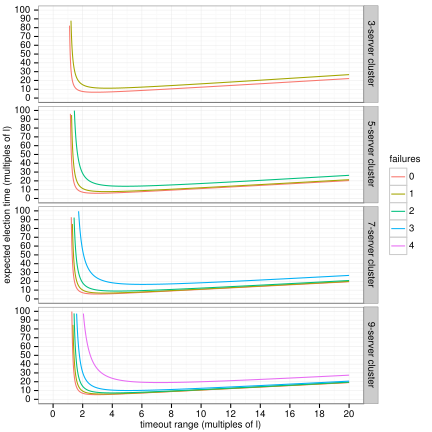
\includegraphics[height=5.5in]{leaderelection/overall}
\hspace{-2em}
\vcaption[expected overall election time]{
The expected total election times for various clusters,
as defined by $\Ex[E_s]$, with a fixed one-way network latency.
It excludes the time to write to stable
storage (which is usually negligible). The timeout range and
expected overall election time are presented as multiples of the one-way
network latency ($l$), since $l$ is typically fixed in a given
deployment.
}
\label{fig:leaderelection:theory:overall}
\end{figure}

Figure~\ref{fig:leaderelection:theory:overall} plots the expected time to
elect a leader when the network latency is fixed, by combining the
formula for $\Ex[E_s]$ with the formula for $Pr(D_{c,s} \leq l)$.
From the graphs, a Raft cluster with a sufficiently broad timeout range
will usually elect a leader within 20 times the one-way network latency,
even when running with a bare majority of available servers. This
suggests that most datacenter Raft deployments should be able to achieve
typical leader election times under \SI{100}{\milli\second}. Even worst
case global deployments, with one-way latencies of
\SI{200}{\milli\second},
should be able to typically elect leaders within \SI{4}{seconds}. (Election
times may be larger if some servers are deployed on other planets.)

Each of the curves has a knee. If the timeout range is chosen to be too
short, too many servers time out before others are able to collect
votes, resulting in poor election times. Once timeout ranges are
sufficiently large (about 3--8 times the network latency, depending on
the cluster), the curves become linear with a slight upward slope:
elections complete after few or no split votes, but they must wait
longer for each timeout to elapse.

The graphs provide insight into how to configure election timeouts: a
conservative setting is probably best in practice. The minimum point on
the graphs represents the best average election time possible for each
given cluster configuration. However, attaining this minimum time is
quite risky, since the minimum is close to the knee in the curve. If the
network latency turns out to be slightly higher than anticipated in
practice, that might push the system into the left region of the graph
where election times skyrocket. It is better to configure systems
farther to the right, trading off a slightly higher average election
time in exchange for a more robust system. Thus, we recommend using a
timeout range that is ten times the one-way network latency (even if the
true network latency is five times greater than anticipated, most clusters would
still be able to elect a leader in a timely manner).
